
\documentclass[letterpaper,hide notes,xcolor={table,svgnames},pdftex,10pt]{beamer}
\def\showexamples{t}

\usecolortheme{crane}
\setbeamertemplate{navigation symbols}{}

\usetheme{MyPittsburgh}
\usepackage{hyperref}
\usepackage{graphicx,xspace}
\usepackage[normalem]{ulem}
\usepackage{multicol}
\usepackage{amsmath,amssymb,amsthm,graphicx,xspace}
\newcommand\SF[1]{$\bigstar$\footnote{SF: #1}}

\usepackage[sfdefault,lf]{carlito}
\usepackage[T1]{fontenc}
\usepackage[scaled]{beramono}
\usepackage{tikzpagenodes}
\newcommand{\Rplus}{\protect\hspace{-.1em}\protect\raisebox{.35ex}{\small{\small\textbf{+}}}}
\newcommand{\Cpp}{\mbox{C\Rplus\Rplus}\xspace}

\newcounter{tmpnumSlide}
\newcounter{tmpnumNote}

\newcommand\mnote[1]{%
	\addtocounter{tmpnumSlide}{1}
	\ifdefined\showcues {~\tiny\fbox{\arabic{tmpnumSlide}}}\fi
	\note{\setlength{\parskip}{1ex}\addtocounter{tmpnumNote}{1}\textbf{\Large \arabic{tmpnumNote}:} {#1\par}}}

\newcommand\mmnote[1]{\note{\setlength{\parskip}{1ex}#1\par}}


\newcommand\mquestion[2]{{~\color{red}\fbox{?}}\note{\setlength{\parskip}{1ex}\par{\Large \textbf{?}} #1} \note{\setlength{\parskip}{1ex}\par{\Large \textbf{A}} #2\par}\ifdefined \presentationonly \pause \fi}

\newcommand\blackboard[1]{%
	\ifdefined   \showblackboard
		{#1}
	\else {\begin{center} \fbox{\colorbox{blue!30}{%
						\begin{minipage}{.95\linewidth}%
							\hspace{\stretch{1}} Some space intentionally left blank; done at the blackboard.%
						\end{minipage}}}\end{center}}%
	\fi%
}

\usepackage{listings}
\lstset{%
	keywordstyle=\bfseries,
	aboveskip=15pt,
	belowskip=15pt,
	captionpos=b,
	identifierstyle=\ttfamily,
	frame=lines,
	numbers=left, basicstyle=\scriptsize, numberstyle=\tiny, stepnumber=0, numbersep=2pt}

\usepackage{siunitx}
\newcommand\sius[1]{\num[group-separator = {,}]{#1}\si{\micro\second}}
\newcommand\sims[1]{\num[group-separator = {,}]{#1}\si{\milli\second}}
\newcommand\sins[1]{\num[group-separator = {,}]{#1}\si{\nano\second}}
\sisetup{group-separator = {,}, group-digits = true}

%% -------------------- tikz --------------------
\usepackage{tikz}
\usetikzlibrary{positioning}
\usetikzlibrary{arrows,backgrounds,automata,decorations.shapes,decorations.pathmorphing,decorations.markings,decorations.text}

\tikzstyle{place}=[circle,draw=blue!50,fill=blue!20,thick, inner sep=0pt,minimum size=6mm]
\tikzstyle{transition}=[rectangle,draw=black!50,fill=black!20,thick, inner sep=0pt,minimum size=4mm]

\tikzstyle{block}=[rectangle,draw=black, thick, inner sep=5pt]
\tikzstyle{bullet}=[circle,draw=black, fill=black, thin, inner sep=2pt]

\tikzstyle{pre}=[<-,shorten <=1pt,>=stealth',semithick]
\tikzstyle{post}=[->,shorten >=1pt,>=stealth',semithick]
\tikzstyle{bi}=[<->,shorten >=1pt,shorten <=1pt, >=stealth',semithick]

\tikzstyle{mut}=[-,>=stealth',semithick]

\tikzstyle{treereset}=[dashed,->, shorten >=1pt,>=stealth',thin]

\usepackage{ifmtarg}
\usepackage{xifthen}
\makeatletter
% new counter to now which frame it is within the sequence
\newcounter{multiframecounter}
% initialize buffer for previously used frame title
\gdef\lastframetitle{\textit{undefined}}
% new environment for a multi-frame
\newenvironment{multiframe}[1][]{%
	\ifthenelse{\isempty{#1}}{%
		% if no frame title was set via optional parameter,
		% only increase sequence counter by 1
		\addtocounter{multiframecounter}{1}%
	}{%
		% new frame title has been provided, thus
		% reset sequence counter to 1 and buffer frame title for later use
		\setcounter{multiframecounter}{1}%
		\gdef\lastframetitle{#1}%
	}%
	% start conventional frame environment and
	% automatically set frame title followed by sequence counter
	\begin{frame}%
		\frametitle{\lastframetitle~{\normalfont(\arabic{multiframecounter})}}%
		}{%
	\end{frame}%
}
\makeatother

\makeatletter
\newdimen\tu@tmpa%
\newdimen\ydiffl%
\newdimen\xdiffl%
\newcommand\ydiff[2]{%
	\coordinate (tmpnamea) at (#1);%
	\coordinate (tmpnameb) at (#2);%
	\pgfextracty{\tu@tmpa}{\pgfpointanchor{tmpnamea}{center}}%
	\pgfextracty{\ydiffl}{\pgfpointanchor{tmpnameb}{center}}%
	\advance\ydiffl by -\tu@tmpa%
}
\newcommand\xdiff[2]{%
	\coordinate (tmpnamea) at (#1);%
	\coordinate (tmpnameb) at (#2);%
	\pgfextractx{\tu@tmpa}{\pgfpointanchor{tmpnamea}{center}}%
	\pgfextractx{\xdiffl}{\pgfpointanchor{tmpnameb}{center}}%
	\advance\xdiffl by -\tu@tmpa%
}
\makeatother
\newcommand{\copyrightbox}[3][r]{%
	\begin{tikzpicture}%
		\node[inner sep=0pt,minimum size=2em](ciimage){#2};
		\usefont{OT1}{phv}{n}{n}\fontsize{4}{4}\selectfont
		\ydiff{ciimage.south}{ciimage.north}
		\xdiff{ciimage.west}{ciimage.east}
		\ifthenelse{\equal{#1}{r}}{%
			\node[inner sep=0pt,right=1ex of ciimage.south east,anchor=north west,rotate=90]%
			{\raggedleft\color{black!50}\parbox{\the\ydiffl}{\raggedright{}#3}};%
		}{%
			\ifthenelse{\equal{#1}{l}}{%
				\node[inner sep=0pt,right=1ex of ciimage.south west,anchor=south west,rotate=90]%
				{\raggedleft\color{black!50}\parbox{\the\ydiffl}{\raggedright{}#3}};%
			}{%
				\node[inner sep=0pt,below=1ex of ciimage.south west,anchor=north west]%
				{\raggedleft\color{black!50}\parbox{\the\xdiffl}{\raggedright{}#3}};%
			}
		}
	\end{tikzpicture}
}


%% --------------------

%\usepackage[excludeor]{everyhook}
%\PushPreHook{par}{\setbox0=\lastbox\llap{MUH}}\box0}

%\vspace*{\stretch{1}

%\setbox0=\lastbox \llap{\textbullet\enskip}\box0}

\setlength{\parskip}{\fill}

\newcommand\noskips{\setlength{\parskip}{1ex}}
\newcommand\doskips{\setlength{\parskip}{\fill}}

\newcommand\xx{\par\vspace*{\stretch{1}}\par}
\newcommand\xxs{\par\vspace*{2ex}\par}
\newcommand\tuple[1]{\langle #1 \rangle}
\newcommand\code[1]{{\sf \footnotesize #1}}
\newcommand\ex[1]{\uline{Example:} \ifdefined \presentationonly \pause \fi
	\ifdefined\showexamples#1\xspace\else{\uline{\hspace*{2cm}}}\fi}

\newcommand\ceil[1]{\lceil #1 \rceil}


\AtBeginSection[]
{
	\begin{frame}
		\frametitle{Outline}
		\tableofcontents[currentsection]
	\end{frame}
}



\pgfdeclarelayer{edgelayer}
\pgfdeclarelayer{nodelayer}
\pgfsetlayers{edgelayer,nodelayer,main}

\tikzstyle{none}=[inner sep=0pt]
\tikzstyle{rn}=[circle,fill=Red,draw=Black,line width=0.8 pt]
\tikzstyle{gn}=[circle,fill=Lime,draw=Black,line width=0.8 pt]
\tikzstyle{yn}=[circle,fill=Yellow,draw=Black,line width=0.8 pt]
\tikzstyle{empty}=[circle,fill=White,draw=Black]
\tikzstyle{bw} = [rectangle, draw, fill=blue!20,
text width=4em, text centered, rounded corners, minimum height=2em]

\newcommand{\CcNote}[1]{% longname
	This work is licensed under the \textit{Creative Commons #1 3.0 License}.%
}
\newcommand{\CcImageBy}[1]{%
	\includegraphics[scale=#1]{creative_commons/cc_by_30.pdf}%
}
\newcommand{\CcImageSa}[1]{%
	\includegraphics[scale=#1]{creative_commons/cc_sa_30.pdf}%
}
\newcommand{\CcImageNc}[1]{%
	\includegraphics[scale=#1]{creative_commons/cc_nc_30.pdf}%
}
\newcommand{\CcGroupBySa}[2]{% zoom, gap
	\CcImageBy{#1}\hspace*{#2}\CcImageNc{#1}\hspace*{#2}\CcImageSa{#1}%
}
\newcommand{\CcLongnameByNcSa}{Attribution-NonCommercial-ShareAlike}

\newenvironment{changemargin}[1]{% 
	\begin{list}{}{% 
		\setlength{\topsep}{0pt}% 
		\setlength{\leftmargin}{#1}% 
		\setlength{\rightmargin}{1em}
		\setlength{\listparindent}{\parindent}% 
		\setlength{\itemindent}{\parindent}% 
		      \setlength{\parsep}{\parskip}% 
		      }% 
		\item[]}{\end{list}}




\title{Lecture 12 --- Threads and Concurrency }

\author{Jeff Zarnett \\ \small \texttt{jzarnett@uwaterloo.ca}}
\institute{Department of Electrical and Computer Engineering \\
	University of Waterloo}
\date{\today}


\begin{document}

\begin{frame}
	\titlepage
\end{frame}


\begin{frame}
	\frametitle{Thread Cancellation}

	Thread cancellation is exactly what it sounds like: a running thread will be terminated before it has finished its work.

	The thread that we are going to cancel is called the \textit{target}.

	\begin{center}
		
\includegraphics[width=0.5\textwidth]{images/canceled_flight.jpg}
	\end{center}

\end{frame}


\begin{frame}[fragile]
	\frametitle{Cancellation Type}

	\begin{enumerate}
		\item \textbf{Asynchronous Cancellation}
		\item \textbf{Deferred Cancellation}
	\end{enumerate}

	thread can declare its own cancellation type through the use of the function:
	\begin{lstlisting}[language=C]
pthread_setcanceltype( int type, int *oldtype )
\end{lstlisting}

	\texttt{type}: \texttt{PTHREAD\_CANCEL\_DEFERRED} or \texttt{PTHREAD\_CANCEL\_ASYNCHRONOUS}

	\texttt{oldtype}: previous state, if we care.

\end{frame}

\begin{frame}
	\frametitle{Send Cancellation}

	The pthread command to cancel a thread is \texttt{pthread\_cancel} and it takes one parameter (the thread identifier).

	To check if the current thread has been cancelled, the function call is \texttt{pthread\_testcancel} which takes no parameters.

	It's polite to check this, if it's a risk.

\end{frame}


\begin{frame}
	\frametitle{Cancellation Points}
	A  large number of functions are \alert{cancellation points}.

	That is, the POSIX specification requires there is an implicit check for cancellation when calling one of those functions.

	Even more are ``potential cancellation points'' -- maybe, maybe not?

\end{frame}



\begin{frame}
	\frametitle{Not Now!}
	Sometimes a thread could die before it has cleaned up.

	\begin{center}
		
\includegraphics[width=0.5\textwidth]{images/tenthdoctor.jpeg}
	\end{center}

	This can leave memory allocated, things locked...

\end{frame}


\begin{frame}[fragile]
	\frametitle{Cleanup Handler}

	We can prevent this with cancellation handlers.

	The functions for cleaning up are:

	\begin{lstlisting}[language=C]
/* Register cleanup handler, with argument */ 
pthread_cleanup_push( void (*routine)(void*), void *argument ); 
/* Run if execute is non-zero */ 
pthread_cleanup_pop( int execute ); 
\end{lstlisting}

	The push function always needs to be paired with the pop function at the same level in your program (where level is defined by the curly braces).

\end{frame}


\begin{frame}[fragile]
	\frametitle{Don't You Forget About Me}

	Consider the following code:
	\begin{lstlisting}[language=C]
void* do_work( void* argument ) {
  struct job * j = malloc( sizeof( struct job ) );
  /* Do something useful with this structure */
  /* Actual work to do not shown */
  free( j );
  pthread_exit( NULL );
\end{lstlisting}


\end{frame}



\begin{frame}[fragile]
	\frametitle{Don't You Forget About me}

	\begin{lstlisting}[language=C]
void cleanup( void* mem ) {
  free( mem );
}

void* do_work( void* argument ) {
  struct job * j = malloc( sizeof( struct job ) );
  pthread_cleanup_push( cleanup, j );
  /* Do something useful with this structure */
  /* Actual work to do not shown */
  free( j );
  pthread_cleanup_pop( 0 ); /* Don't run */
  pthread_exit( NULL );
\end{lstlisting}


\end{frame}


\begin{frame}
	\frametitle{Ah! Ah! Ah!}

	Next, we'l; do an example where we don't use the return value of a thread, but do use attributes.

	For the sake of simplicity: we are just going to count!

	\begin{center}
		
\includegraphics[width=0.6\textwidth]{images/countvoncount.jpg}
	\end{center}


\end{frame}



\begin{frame}[fragile]
	\frametitle{Slightly Larger Example}

	\begin{lstlisting}[language=C]
#include <pthread.h>
#include <stdio.h>

int sum; /* Shared Data */

void *runner(void *param);

int main( int argc, char **argv ) {
  pthread_t tid; /* the thread identifier */
  pthread_attr_t attr; /* set of thread attributes */

  if ( argc != 2 ) {
    fprintf(stderr,"usage: %s <integer value>\n", argv[0]); 
    return -1;
  }
  if ( atoi( argv[1] ) < 0 ) {
    fprintf(stderr, "%d must be >= 0\n", atoi(argv[1])); 
    return -1;
  }

  pthread_attr_init( &attr ); /* set the default attributes */
  pthread_create( &tid, &attr, runner, argv[1] ); /* create the thread */
  pthread_join( tid, NULL ); 
  printf( "sum = %d\n", sum );
  pthread_exit( NULL );
}
\end{lstlisting}


\end{frame}

\begin{frame}[fragile]
	\frametitle{Slightly Larger Example}


	\begin{lstlisting}[language=C]
void *runner( void *param ) {
  int upper = atoi( param );
  sum = 0;
  for ( int i = 1; i <= upper; i++ ) {
    sum += i;
  }
  pthread_exit( 0 );
}
\end{lstlisting}

	In this example, both threads are sharing the global variable \texttt{sum}.

	Do we have coordination?

\end{frame}


\begin{frame}
	\frametitle{Coordination, Count to 10}
	Yes! The parent thread will join the newly-spawned thread (i.e., wait until it is finished) before it tries to print out the value.

	If it did not, the parent would print the sum early.

	Let's do a different take on that program.

	\begin{center}
		
\includegraphics[width=0.6\textwidth]{images/sesamestreet.png}
	\end{center}

\end{frame}

\begin{frame}[fragile]
	\frametitle{Slightly Larger Example 2}

	\begin{lstlisting}[language=C]
#include <pthread.h>
#include <stdio.h>
#include <stdlib.h>

int sum = 0;

void* runner( void *param ) {
    int upper = atoi( param );
    for (int i = 1; i <= upper; i++ ) {
        sum += i;
    }
    pthread_exit( 0 );
}
\end{lstlisting}


\end{frame}

\begin{frame}[fragile]
	\frametitle{Slightly Larger Example 2}


	\begin{lstlisting}[language=C]
int main( int argc, char** argv ) { 

    pthread_t tid[3];

    if ( argc != 2 ) {
        printf("An integer value is required as an argument.\n");
        return -1; 
    }   
    if ( atoi( argv[1]) < 0 ) {
        printf( "%d must be >= 0.\n", atoi(argv[1]) );
    }   

    for ( int i = 0; i < 3; ++i ) { 
        pthread_create( &tid[i], NULL, runner, argv[1] );
    }   
    for ( int j = 0; j < 3; ++j ) { 
        pthread_join( tid[j], NULL );
    }   
    printf( "sum = %d.\n", sum );
    
    pthread_exit( 0 );
}
\end{lstlisting}

	What happens when we run this program?

\end{frame}


\begin{frame}
	\frametitle{Sometimes...}

	For very small values of the argument, nothing goes wrong.

	For a large number we get some strange and inconsistent results. Why?

	There are three threads that are modifying \texttt{sum}.

	But what does ``at the same time'' mean?

\end{frame}

\begin{frame}
	\frametitle{Multiprocessing}

	Not that long ago, a typical computer had one processor with one core.

	It could accordingly do exactly one thing at a time.

	1 processor: 1 general purpose processor that executes user processes.

	There may be special-purpose processors in the system (RAID controller).

	Only one general purpose processor so we call it a uniprocessor system.



\end{frame}


\begin{frame}
	\frametitle{Multiprocessing}

	Now, desktops, laptops, and even cell phones are using multi-core processors.

	A quad-core processor may be executing four different instructions from four different threads at the same time.

	In theory, multiple processors may mean that we can get more work done in the same amount of (wall clock) time, but this is not a guarantee.

\end{frame}


\begin{frame}
	\frametitle{Terminology Note}


	Terminology note: we often refer to a logical processing unit as a \alert{core}.

	CPU may refer to a physical chip that contains 1+ logical processing units.

	As far as the operating system is concerned, it does not much matter if a system has four cores in four physical chips or four cores in one chip.

	Either way, there are four units that can execute instructions.



\end{frame}


\begin{frame}
	\frametitle{Execution}

	1 process, 1 thread: it does not matter how many cores are available.\\
	\quad At most one core will be used to execute this task.

	If there are multiple processes, each process can execute on a different core.

	But what if there are more processes and threads than available cores?

	We can hope that the processes get blocked frequently enough and long enough?



\end{frame}


\begin{frame}
	\frametitle{Chest Day Best Day}

	\begin{center}
		
\includegraphics[width=0.5\textwidth]{images/chestdaybestday.png}
	\end{center}

	``Can I work in with you?''

\end{frame}


\begin{frame}
	\frametitle{Execution}


	Switch between the different tasks via a procedure we call \alert{time slicing}.

	So thread 1 would execute for a designated period, such as 20 ms, then thread 2 for 20 ms, then thread 3 for 20 ms, then back to thread 1 for 20 ms.

	To the user, it seems like threads 1, 2, and 3 are being executed in parallel.\\
	\quad 20 ms is fast enough that the user does not notice the difference.

\end{frame}


\begin{frame}
	\frametitle{Single Core Execution}

	\begin{center}
		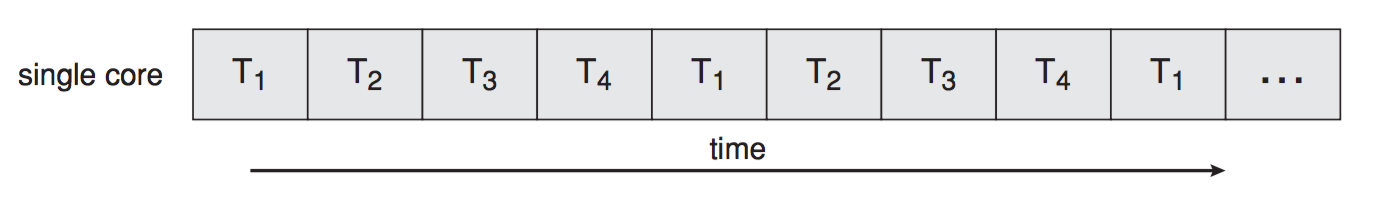
\includegraphics[width=\textwidth]{images/single-core-execution.png}
	\end{center}

\end{frame}


\begin{frame}
	\frametitle{Multi Core Execution}

	Time slicing will still occur, if necessary:

	\begin{center}
		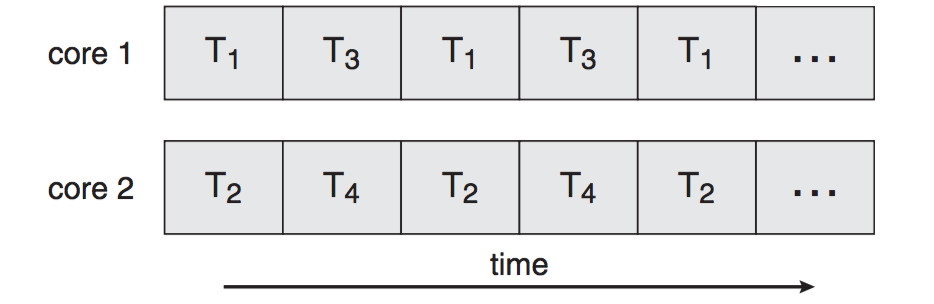
\includegraphics[width=\textwidth]{images/dual-core-execution.png}
	\end{center}


\end{frame}



\begin{frame}
	\frametitle{Parallelism}

	Multiple threads at the same time = tasks completed faster?

\end{frame}

\begin{frame}
	\frametitle{Parallelism and Speedup}

	Depends on the nature of the task!

	Fully parallelized: 2 $\times$ Threads = 2 $\times$ Speed

	Partially parallelized: 2 $\times$ Threads = $(1 < n < 2)$ $\times$ Speed

	Cannot be parallelized: 2 $\times$ Threads = $1$ $\times$ Speed

\end{frame}


\begin{frame}
	\frametitle{Heard, Chef!}

	\begin{center}
		
\includegraphics[width=\textwidth]{images/lamb-sauce.jpg}
	\end{center}

\end{frame}



\begin{frame}
	\frametitle{Speedup Example}


	Suppose: a task that can be executed in 5~s, containing a parallelizable loop.

	Initialization and recombination code in this routine requires 400~ms.

	So with one processor executing, it would take about 4.6~s to execute the loop.

	Split it up and execute on two processors: about 2.3~s to execute the loop.

	Add to that the setup and cleanup time of 0.4~s and we get a total time of 2.7~s.

	Completing the task in 2.7~s rather than 5~s represents a speedup of about~46\%.

\end{frame}


\begin{frame}
	\frametitle{Amdahl's Law}

	Gene Amdahl came up with a formula for the general case of how much faster a task can be completed based on how many processors we have available.

	Let us define $S$ as the portion of the application that must be performed serially and $N$ as the number of processing cores available.

	Amdahl's Law:

	\begin{center}
		speedup $\leq$ {\huge $\frac{1}{S + \frac{1-S}{N}}$}
	\end{center}

\end{frame}


\begin{frame}
	\frametitle{Amdahl's Law}

	Take the limit as $N \rightarrow$ infinity and you will find the speedup converges to $\frac{1}{S}$.


	The limiting factor on how much additional processors help is the size of $S$.

	Matches our intuition of how it should work.

\end{frame}


\begin{frame}
	\frametitle{Amdahl's Law on the 5~s Task}

	Applying this formula to the example from earlier:

	\begin{center}
		\begin{tabular}{l|l}
			\textbf{Processors} & \textbf{Run Time (s)} \\ \hline
			1                   & 5                     \\
			2                   & 2.7                   \\
			4                   & 1.55                  \\
			8                   & 0.975                 \\
			16                  & 0.6875                \\
			32                  & 0.54375               \\
			64                  & 0.471875              \\
			128                 & 0.4359375             \\
		\end{tabular}
	\end{center}

\end{frame}


\begin{frame}
	\frametitle{Observations on the 5~s Task}

	1. Diminishing returns as we add more processors.

	2. Converges on 0.4~s.

	The most we could speed up this code is by a factor of $\frac{5}{0.4}\approx 12.5$.

	But that would require infinite processors (and therefore infinite money).

\end{frame}


\begin{frame}
	\frametitle{Merge Sort Example}

	Recall from data structures and algorithms the concept of merge sort.

	This is a divide-and-conquer algorithm like binary search.

	Split the array of values up into smaller pieces, sort those, and then merge the smaller pieces together to have sorted data.


\end{frame}


\begin{frame}
	\frametitle{Merge Sort Example}

	\begin{center}
		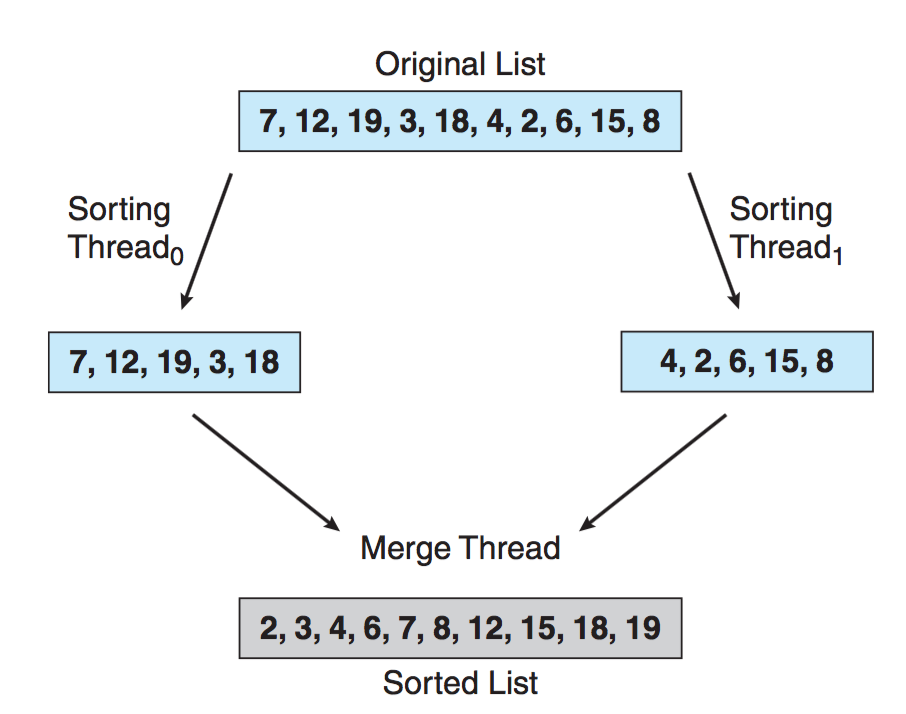
\includegraphics[width=0.75\textwidth]{images/multithread-sort.png}
	\end{center}


\end{frame}



\end{document}

